\documentclass{beamer}

% --------------------------------------------------
% Packages and Bibliography
% --------------------------------------------------
\usepackage{hyperref}
\usepackage{adjustbox}
\usepackage{float}
\floatplacement{algorithm}{H}
\usepackage{algorithm}
\usepackage{algorithmicx}
\usepackage{algcompatible}
\usepackage{algpseudocode}
\usepackage[normalem]{ulem}        % for underlining, strikeout
\usepackage{subcaption}
% Bibliography
\usepackage[backend=biber, style=numeric, sorting=none, doi=true, url=true]{biblatex}
\addbibresource{ref.bib}

% --------------------------------------------------
% XeLaTeX and CJK Fonts
% --------------------------------------------------
\usepackage[CJKmath=true, AutoFakeBold=true]{xeCJK}
\setCJKmainfont{AR PL KaitiM Big5}
\setCJKsansfont{AR PL KaitiM Big5}
\setCJKmonofont{AR PL KaitiM Big5}
\newCJKfontfamily\Kai{標楷體}
\XeTeXlinebreaklocale "zh"

% --------------------------------------------------
% Fonts, Colors, and Theme
% --------------------------------------------------
\usepackage[T1]{fontenc}
\usepackage{latexsym, amssymb, amsfonts, amsmath, amsthm, mathrsfs, mathptmx}
\usepackage{graphicx, pstricks}
\usepackage{tikz}
\usetikzlibrary{arrows.meta, positioning}
\usepackage{multicol}
\usepackage{booktabs}
\usepackage{calligra}
\usepackage{soul}
\usepackage{enumitem}
\usefonttheme[onlymath]{serif}

% Code listings
\usepackage{listings}
\lstset{
    language=[LaTeX]TeX,
    basicstyle=\ttfamily\footnotesize,
    keywordstyle=\bfseries\color[RGB]{0,0,139},
    stringstyle=\color[RGB]{50,50,50},
    numbers=left,
    numberstyle=\small\color{gray},
    rulesepcolor=\color{red!20!green!20!blue!20},
    frame=shadowbox,
}

% --------------------------------------------------
% Itemize and Enumerate Customization
% --------------------------------------------------
% Beamer item symbols
\setbeamertemplate{itemize item}{$\bullet$}
\setbeamertemplate{itemize subitem}{--}
\setbeamertemplate{itemize subsubitem}{$\circ$}

% enumitem settings
\setlist[itemize,1]{label=\usebeamertemplate{itemize item}, leftmargin=1.5em, itemsep=0.3em}
\setlist[itemize,2]{label=--, leftmargin=2.5em, labelsep=0.5em, topsep=0.3em, itemsep=0.1em}
\setlist[itemize,3]{label=$\circ$, leftmargin=3em, labelsep=0.5em, topsep=0.3em, itemsep=0.1em}
\setlist[enumerate,1]{label=\arabic*., ref=\arabic*}
\setlist[enumerate,2]{label=\alph*), ref=\theenumi\alph*}

% --------------------------------------------------
% Custom Commands and Metadata
% --------------------------------------------------
\renewcommand{\today}{\number\year 年\number\month 月\number\day 日}
\renewcommand{\alert}[1]{\textbf{\color{swufe}#1}}

% University style
\usepackage{JNU}

% Presentation metadata
\author{陳景龢}
\title{The AI Economist: Taxation policy design via two-level
deep multiagent reinforcement learning}
\institute[NCCU]{\normalsize Econ Dept\quad NCCU}
\date{2025年6月3日}
\begin{document}

    \begin{frame}
        \titlepage
        \begin{figure}[htpb]
            \centering
        \end{figure}
    \end{frame}

    \begin{frame}
        \tableofcontents[sectionstyle=show,subsectionstyle=show/shaded/hide,subsubsectionstyle=show/shaded/hide]
    \end{frame}

    \begin{frame}{General Settings}
        \begin{itemize}
            \item learning environments : one-step v.s Gather trade build 
            \item Design of agent follows Mirrleesian framework
                \begin{itemize}
                    \item agents perform labor $l$ to earn income $z$, $z$ is different because of skill
                    \item agent's utility increases with its posttax income and decreases with its labor
                    \item agents are heterogeneously skilled
                \end{itemize}
        \end{itemize}
        
    \end{frame}
    
    \begin{frame}{Simulation dynamics}
        \begin{itemize}
            \item Taxation
                \begin{itemize}
                    \item Agent pay tax according to tax schedule $T(z, \tau)$
                    \item Tax schedule can chagne at the start of each tax year
                    \item Collected taxes are evenly redistributed back to agents
                \end{itemize}
            \item Behavioral models
                \begin{itemize}
                    \item each actor observes only portion of the full world state $s_t$
                \end{itemize}
        \end{itemize}

    \end{frame}


    \section{Learning Algorithm \& Training tricks}
        \begin{frame}{Learning Algorithm : Two-step RL}
            The Algorithm is called two-step because the Agents (the inner level) need to adapt to policies set and vice versa
            \begin{figure}[h]
            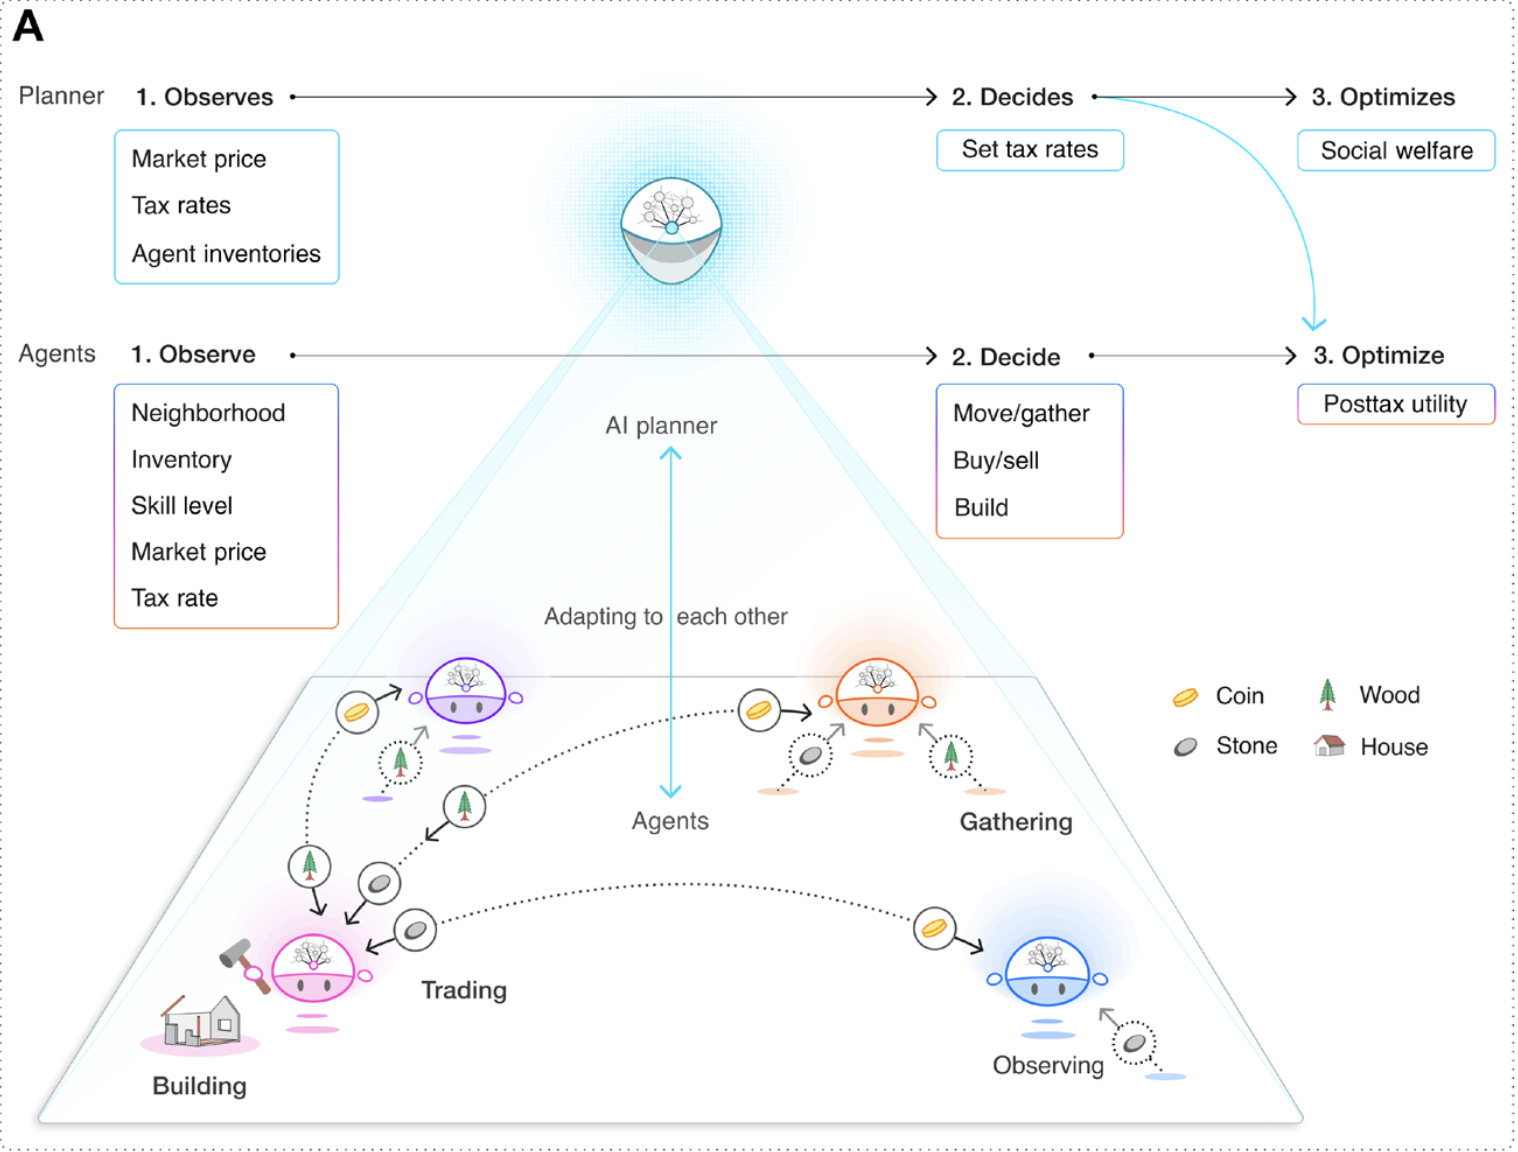
\includegraphics[scale=0.3]{./img/pic1.png}
            \end{figure}
        \end{frame}

        \begin{frame}{Training tricks}
            \begin{itemize}
                \item Curriculum learning
                    \begin{itemize}
                        \item agents adapt to tax schedule then planner starts to learn 
                        \item gradually introduce labor costs and then taxes in a similar way
                    \end{itemize}
                \item Entropy regularization : To stimulate exploration of policy
            \end{itemize}
        \end{frame}

        \begin{frame}{PPO}
            \sout{之後更新}
        \end{frame}

    \section{Learning Environment}

        \subsection{one-step economy}

        \begin{frame}{One-step economy : Basic Settings}
            The one-step economy is a simplifyed Environment which equiped with
            the following properties : 
            \begin{itemize}
                \item planner and the agents each make a
            single decision: The planner sets taxes, and the agents choose an
            amount of labor to perform
                \item the agents decision is indepent from other agents
            \end{itemize}

        \end{frame}

        \begin{frame}{One-step economy : Simulation Results}
            \begin{itemize}
                \item AI Economist can learn simular results to the analytical formula Saez tax
                \item AI Economist can acheive higher social welfare
            \end{itemize}
            \begin{figure}[h]
                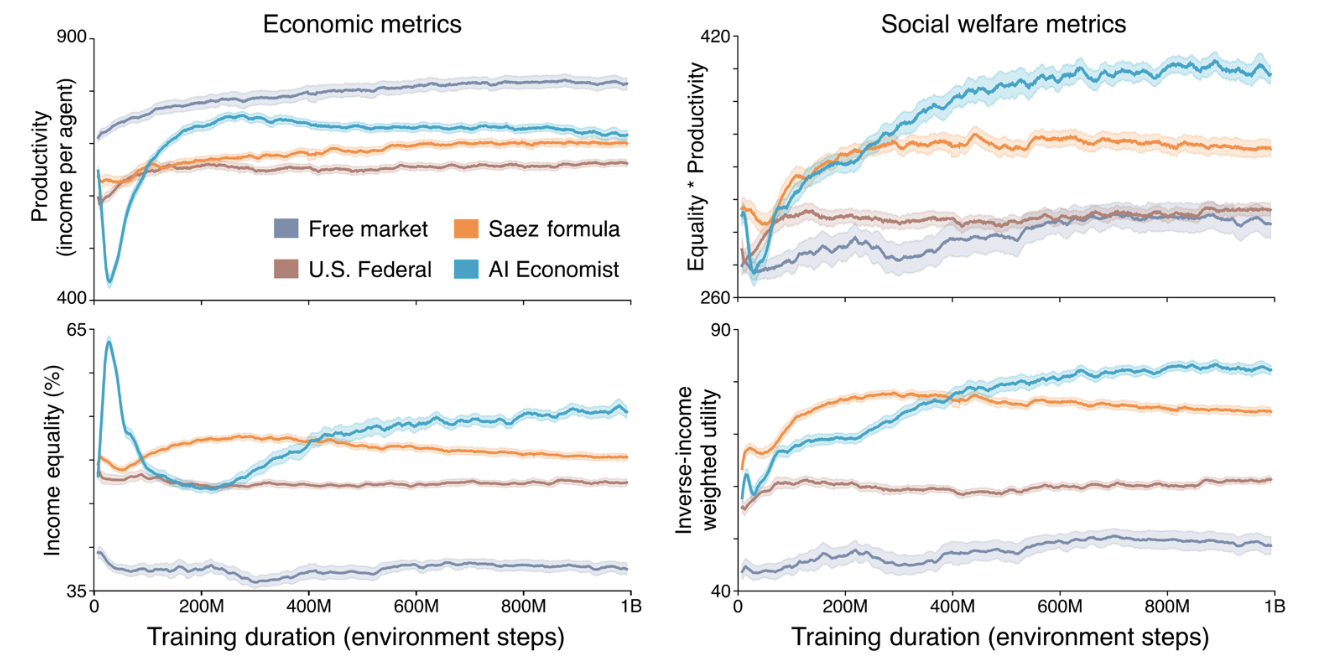
\includegraphics[width=10cm]{./img/pic2.png}
            \end{figure}
        \end{frame}

        \subsection{Gather-Trade-Build: spatiotemporal
    economies}

    \begin{frame}{Gather-Trade-Build : Basic Settings}
        \begin{itemize}
            \item two-dimensional, spatiotemporal economy
            \item agents who move, gather resources (stone and wood), trade, and build houses
        \end{itemize}
        \begin{figure}[h]
            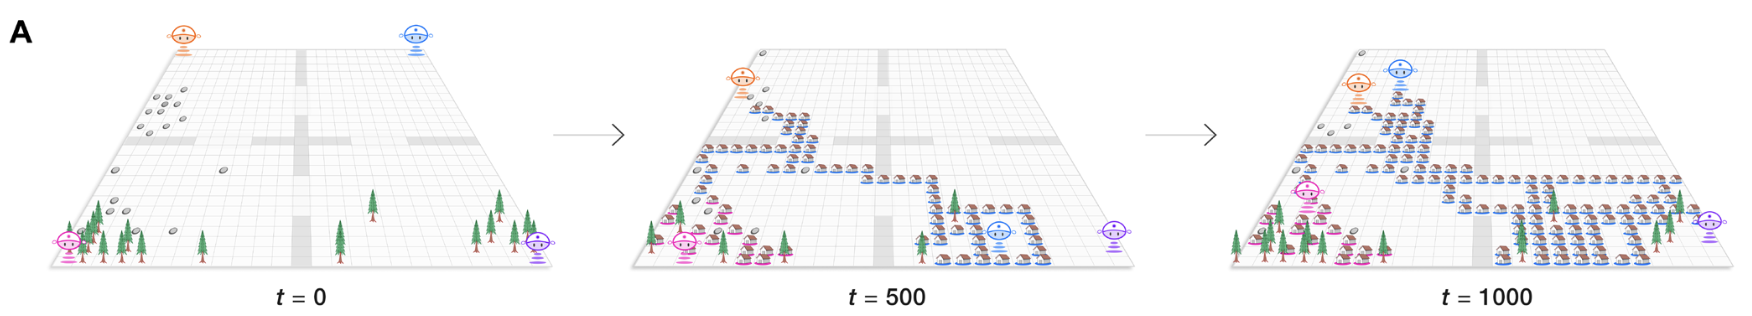
\includegraphics[width=10cm]{./img/pic3.png}
        \end{figure}
        
    \end{frame}

    \begin{frame}{Gather-Trade-Build : Results}
        The micro-level simulation can cause many important economy phenomenon
        \begin{itemize}
            \item Specialization
                \begin{itemize}
                    \item utility-maximizing agents learn to specialize their behavior based on their build-skill
                    \item They earn income by gathering and selling resources
                \end{itemize}
            \begin{figure}[h]
                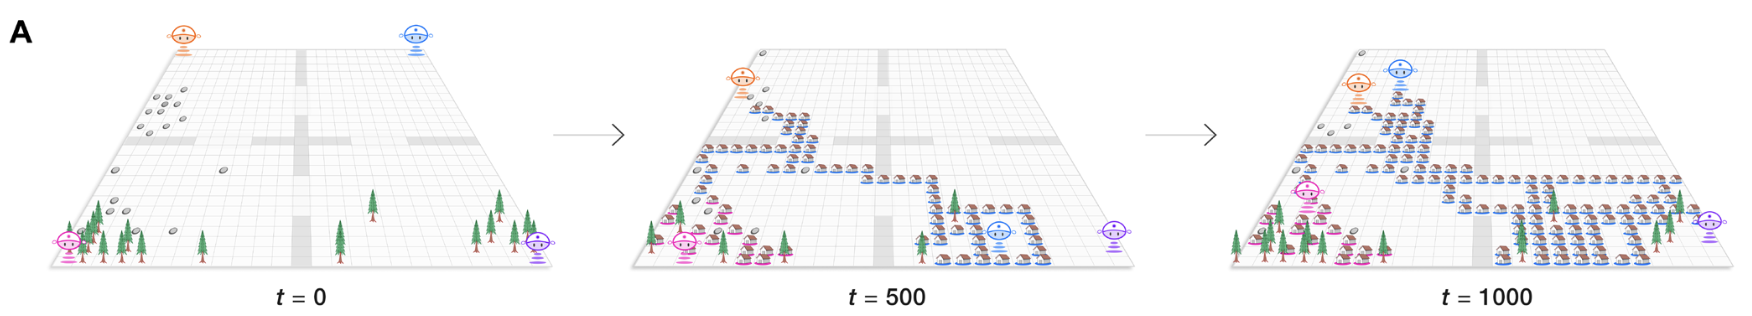
\includegraphics[width=10cm]{./img/pic3.png}
            \end{figure}

        \end{itemize}
    \end{frame}

    \begin{frame}{Con'd}
        \begin{itemize}
            \item Equality-productivity trade-off
                \begin{itemize}
                    \item tax rates $\uparrow \quad \Rightarrow$ Equality $\uparrow$, productivity $\downarrow$
                    \begin{flushleft}
                    \begin{figure}
                        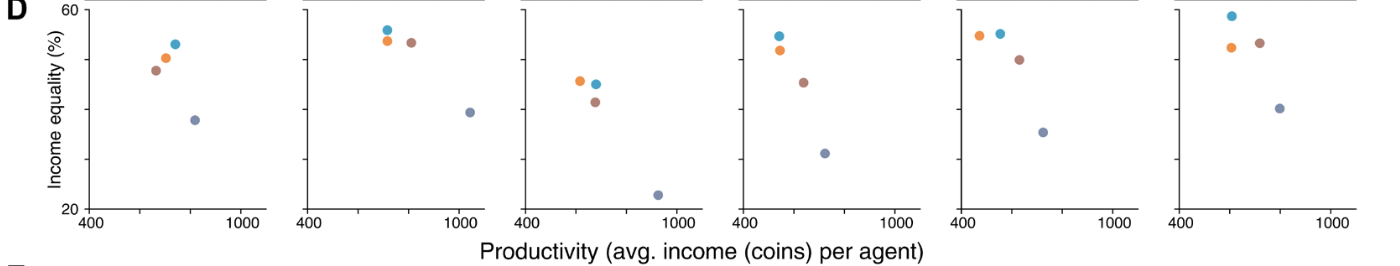
\includegraphics[width=10cm]{./img/pic4.png}
                    \end{figure}
                    \end{flushleft}
                \end{itemize}
            \item tax-gaming strategies
                \begin{itemize}
                    \item agents learn to strategize earning income across tax periods 
                \end{itemize}
            \begin{figure}[htb]
            \setkeys{Gin}{width=0.24\linewidth}
                \subfloat[Figure 1]{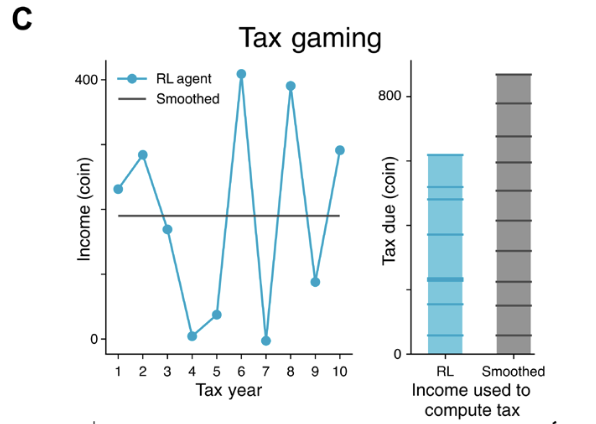
\includegraphics{./img/pic5.png}}
                \subfloat[Figure 2]{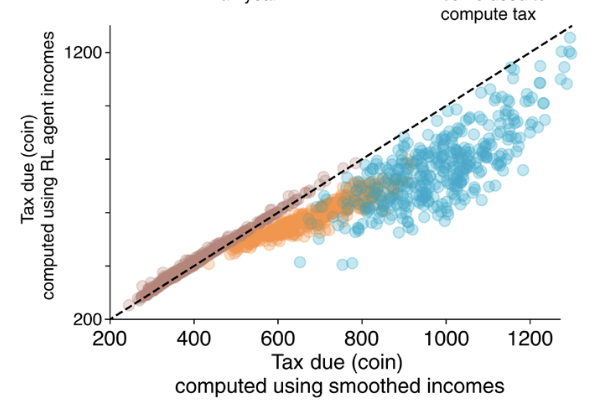
\includegraphics{./img/pic6.png}}
            \end{figure}
        \end{itemize}
        
    \end{frame}

    

\end{document}